\documentclass[../ace.tex]{subfiles}

\begin{document}
\section{Microarchitettura CPU}
\subsection{La CPU}
Una rete logica è definita \textbf{combinatoria} se dati degli ingressi, fornisce sempre gli stessi valori d'uscita, indipendenti dal tempo.
\\
Diversamente una rete \textbf{sequenziale} è una macchina a stati finiti, dotata di memoria, quindi a valori in ingresso corrispondono uscite che dipendenti dallo stato attuale.

Dal punto di vista funzionale è possibile suddividere la CPU in due parti: data path e unità di controllo.
Il data path, di cui componente fondamentale è l'ALU, è una rete logica che si limita ad eseguire istruzioni indicategli dall'unità di controllo, una rete sequenziale di stati: fetch, decode ed execute.

\subsection{Architettura di riferimento RISC}
\begin{figure}[h]
    \centering
    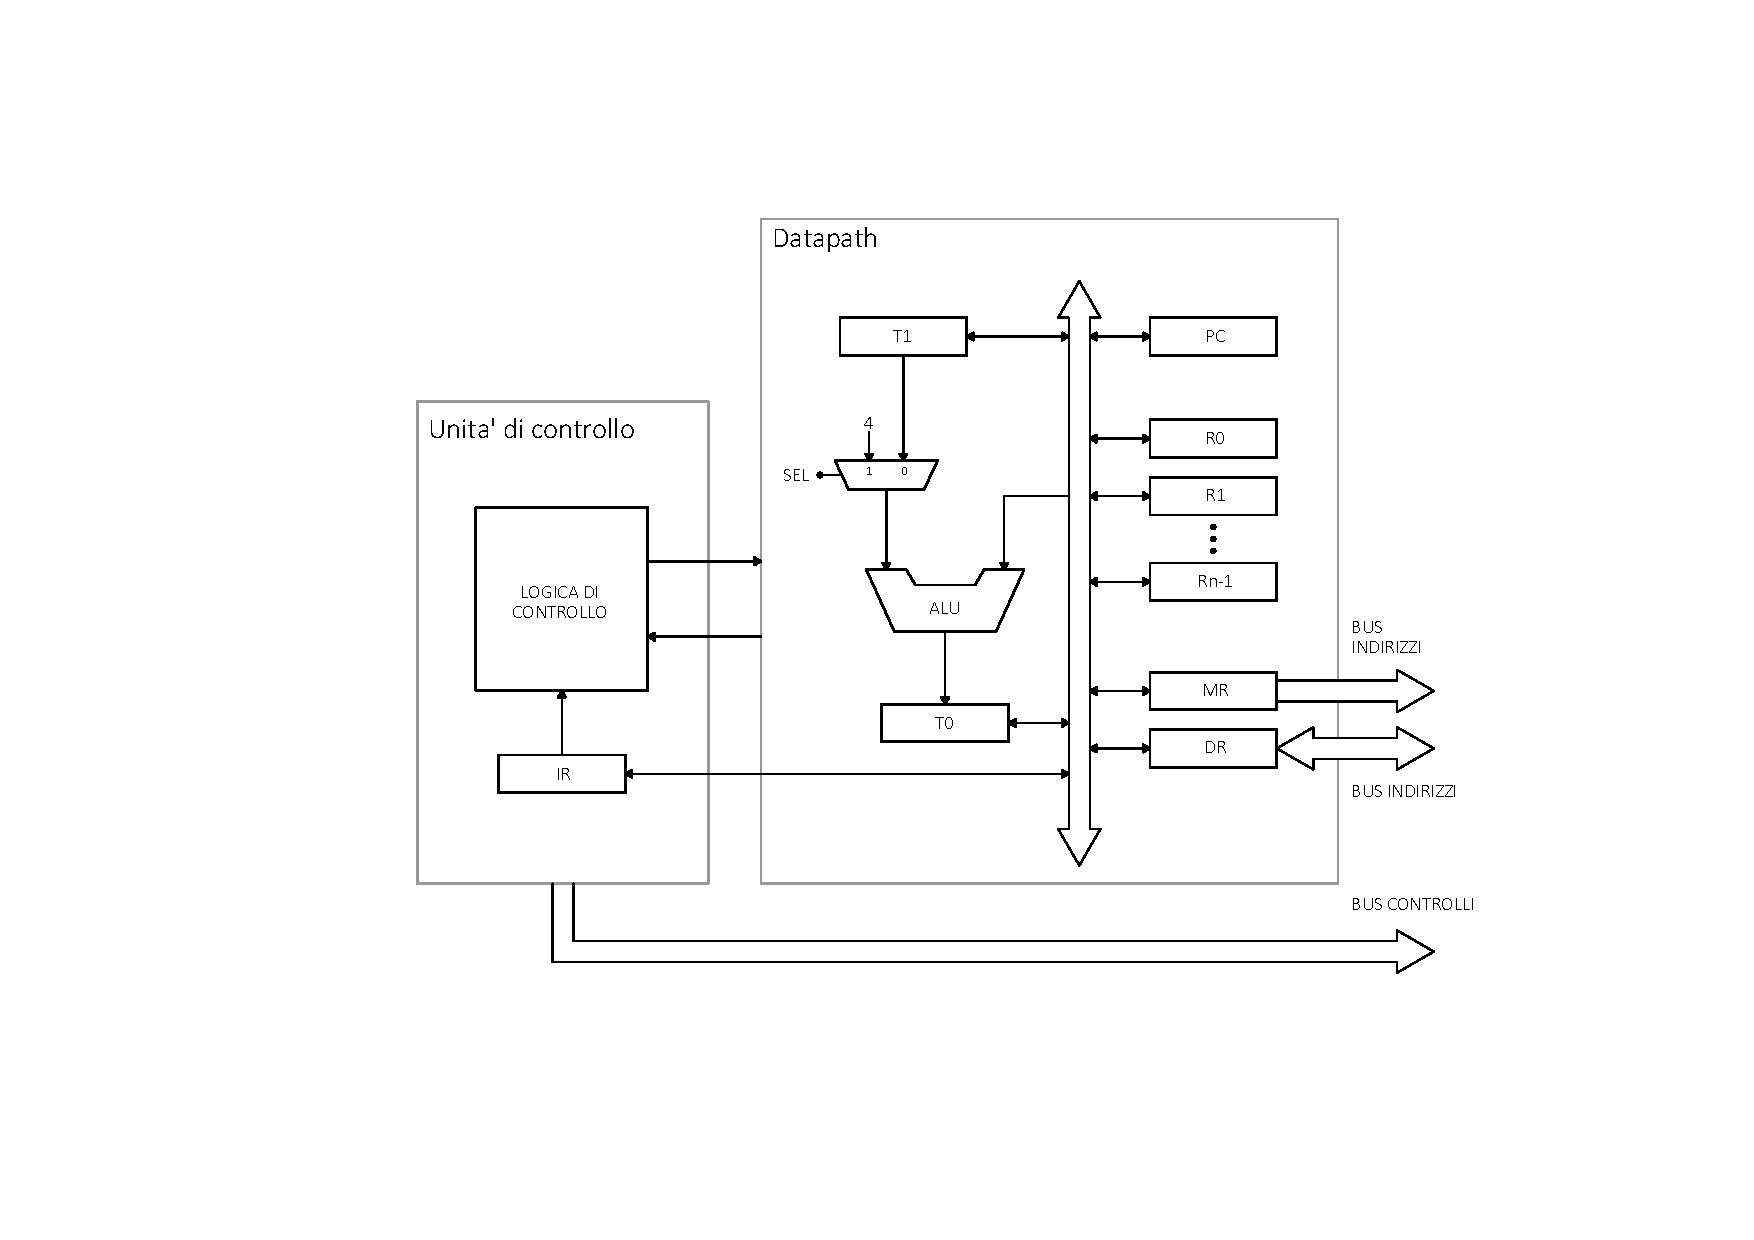
\includegraphics[width=.9\textwidth]{suddivisione_cpu}
\end{figure}
Analizziamo adesso un esempio di architettura RISC.

Un indirizzo indica la posizione di un byte in memoria, ad esempio l'indirizzo 2 indica il secondo byte, posizionato all'ottavo bit.
\\
Le istruzioni sono di lunghezza fissa a 32 bit.
Dato che istruzioni e dati sono salvati sempre ad indirizzi multipli di 4, il program counter è incrementato di 4 ad ogni istruzione.
I registri, a 32bit, sono 32 e di uso generale. L'insieme dei registri prende il nome di register file.

In generale l'esecuzione all'interno di un processore passa attraverso 5 fasi: fetch, decode, execute, memory e writeback.
\\
Nella prima fase (IF) il processore si occupa di leggere dalla memoria l'istruzione indicata dal program counter. Successivamente nella fase di decode (ID) viene decodificata e passata alla fase di execute (EX).
Una volta eseguita, in alcuni casi vengono scritti o letti dei dati dalla memoria (ME), ed infine dove necessario vi è la fase di writeback (WB) dove il risultato dell'operazione è scritta in un registro.

Ogni istruzione di questa ISA di riferimento può appartenere ad una delle tre seguenti categorie:
\begin{itemize}
    \item Istruzione aritmetico/logica \lstinline{add reg1, reg2, dest}
        \begin{figure}[h]
            \centering
            \begin{tikzpicture}[every node/.style={draw, minimum height=.6cm}]
                \node[minimum width=1.8cm](n1) at (0, 0) {opcode};
                \node[right=0pt of n1, minimum width=1.5cm](reg1) {R1};
                \node[right=0pt of reg1, minimum width=1.5cm](reg2) {R2};
                \node[right=0pt of reg2, minimum width=1.5cm](regd) {RD};
                \node[right=0pt of regd, minimum width=3.3cm](opalu){opalu};

                \draw
                    (n1.north) node[anchor=south, draw=none] {\scriptsize 6bit}
                    (reg1.north) node[anchor=south, draw=none] {\scriptsize 5bit}
                    (reg2.north) node[anchor=south, draw=none] {\scriptsize 5bit}
                    (regd.north) node[anchor=south, draw=none] {\scriptsize 5bit}
                    (opalu.north) node[anchor=south, draw=none] {\scriptsize 11bit}
                    ;
            \end{tikzpicture}
        \end{figure}

    \item accesso alla memoria/salto condizionato \lstinline{je  r2,r3,0045h}
        \begin{figure}[h]
            \centering
            \begin{tikzpicture}[every node/.style={draw, minimum height=.6cm}]
                \node[minimum width=1.8cm](n1) at (0, 0) {opcode};
                \node[right=0pt of n1, minimum width=1.5cm](reg1) {R1};
                \node[right=0pt of reg1, minimum width=1.5cm](reg2) {R2};
                \node[right=0pt of reg2, minimum width=4.8cm](offset){offset};
                \draw
                    (n1.north)    node[anchor=south, draw=none]{\scriptsize 6bit}
                    (reg1.north)  node[anchor=south, draw=none]{\scriptsize 5bit}
                    (reg2.north)  node[anchor=south, draw=none]{\scriptsize 5bit}
                    (offset.north)node[anchor=south, draw=none]{\scriptsize 16bit}
                    ;
            \end{tikzpicture}
        \end{figure}
    \item Salti incondizionati \lstinline{jmp 0045h}
        \begin{figure}[h]
            \centering
            \begin{tikzpicture}[every node/.style={draw, minimum height=.6cm}]
                \node[minimum width=1.8cm](n1) at (0, 0) {opcode};
                \node[right=0pt of n1, minimum width=7.8cm](addr) {address};
                \draw
                    (n1.north) node[anchor=south, draw=none]{\scriptsize 6bit}
                    (addr.north) node[anchor=south, draw=none]{\scriptsize 11bit}
                    ;
            \end{tikzpicture}
        \end{figure}
\end{itemize}

Oltre ai salti condizionati ed incondizionati esiste un terzo tipo di salto, la chiamata a funzione: un salto incondizionato che all'invocazione memorizza il valore corrente di \code{PC}, necessario per riprendere l'esecuzione una volta terminate le istruzioni della funzione.
\\
Assumendo che in questa prima architettura non sia presente uno stack
\footnote{Zona di memoria organizzata a pila LIFO, accessibile attraverso le istruzioni \lstinline{push} e \lstinline{pop}}, chiamate a funzione salveranno il valore di \code{PC} nel registro \code{R31}.
%27: ragionamento di funzionamento dell'ALU

Nel componente ALU, l'ingresso \code{OPALU} definisce l'operazione aritmetica da eseguire sui due segnali \code{ALUsorgA} e \code{ALUsorgB}.
Oltre al risultato dell'operazione, in uscita sono presenti anche dei flag che ne descrivono le caratteristiche, come \code{zf} (\textit{Zero Flag}) e \code{sf} (\textit{Sign Flag})  (vedi lista dei flag a pagina \pageref{8086_flags}).

\subsubsection{Load e Store}
%35
Load e store permettono rispettivamente lettura e scrittura in memoria.
Entrambe prendono in ingresso un registro base, uno destinazione ed un offset.
L'indirizzo su cui leggere/scrivere il dato contenuto nel registro destinazione viene ottenuto sommando l'offset al registro base.
Per comunicare con la memoria si passa attraverso un unico bus, controllato da buffer 3state. Per leggere o scrivere è necessario abilitare i segnali
\code{Mread} e \code{Mwrite}.

\subsubsection{Register File}
Prende come ingressi il primo registro (5bit), il secondo registro (5bit), il registro destinazione (5bit) e 32bit che identificano il dato in ingresso.
In uscita ha due porte a 5bit che riportano i dati letti dal registro sorgente 1 e 2.
%49

\def\tmono{T_\text{mono}}
\def\tmulti{T_\text{multi}}
\subsection{CPU monociclo}
% TODO: aggiungere disegno CPU monociclo
In una CPU monociclo, tutte le istruzioni impiegano un unico ciclo di clock. È una struttura molto semplice, ma potenzialmente anche molto
lenta, dato che il tempo di esecuzione di ogni istruzione necessita di essere pari al tempo di esecuzione di quella più lenta.

Facendo riferimento all'istruzione \lstinline{st R6,R1, 20},
dato che in un unico ciclo di clock devo eseguire sia fetch dell'istruzione che store, sono necessarie due memorie separate.
È inevitabile l'uso di un'architettura di Harvard (vedi pagina \pageref{sec:architettura_harvard}).
Oltre alla doppia memoria introdotta dall'architettura è necessario duplicare anche altre risorse, come ad esempio un sommatore , richiesto per incrementare sia valore del program counter siccome l'ALU è già utilizzata in fase di execute.

Tra le varie operazioni dell'ISA, il tempo di esecuzione maggiore è dovuto sicuramente alla \lstinline{load} (vedi tabella \ref{tab:tempi_esecuzione_monociclo}),
che oltre alle fasi di fetch e decode richiede: calcoli dall'ALU, writeback ed accesso alla memoria.
Chiamato il suo tempo di esecuzione $\tmono=82ns$ ed $N$ il numero di istruzioni, il tempo di esecuzione del programma è $\tmono \cdot N$.

\begin{table}[h]
    \centering
    \begin{tabular}{|c|c|c|c|c|c|c|}
        \hline
    & Fetch  & Decode & ALU & Memory & Writeback & Totale \\
    \hline
        Aritm.   & 30 & 5 &  12 &        &         5 &      52\\
        Load     & 30 & 5 &  12 &     30 &         5 &      82\\
        Store    & 30 & 5 &  12 &     30 &           &      77\\
        jmp cond.& 30 & 5 &  12 &        &           &      47\\
        jmp      & 30 & 5 &     &        &           &      35\\
        jal/call & 30 & 5 &     &        &         5 &      40\\
        \hline
    \end{tabular}
    \caption{Esempio tempi di esecuzione in architettura monociclo}
    \label{tab:tempi_esecuzione_monociclo}
\end{table}

% Lezione 2.6
\subsection{CPU multiciclo}
Ogni fase dell'istruzione è eseguita in un ciclo di clock differente.
Alla base di questa architettura c'è il ragionamento che molte delle istruzioni dell'ISA richiedono un tempo di esecuzione notevolmente inferiore rispetto al resto delle istruzioni.
In altre parole, chiamato $\sum\tmulti$ il tempo di esecuzione di una singola istruzione il numero di istruzioni per cui
$\sum\tmulti > \tmono$ sarà inferiore al numero di istruzioni per cui $\sum\tmulti < \tmono$.
Ne consegue che l'architettura multiciclo è mediamente più veloce di un architettura monociclo.

\begin{figure}[h]
    \centering
    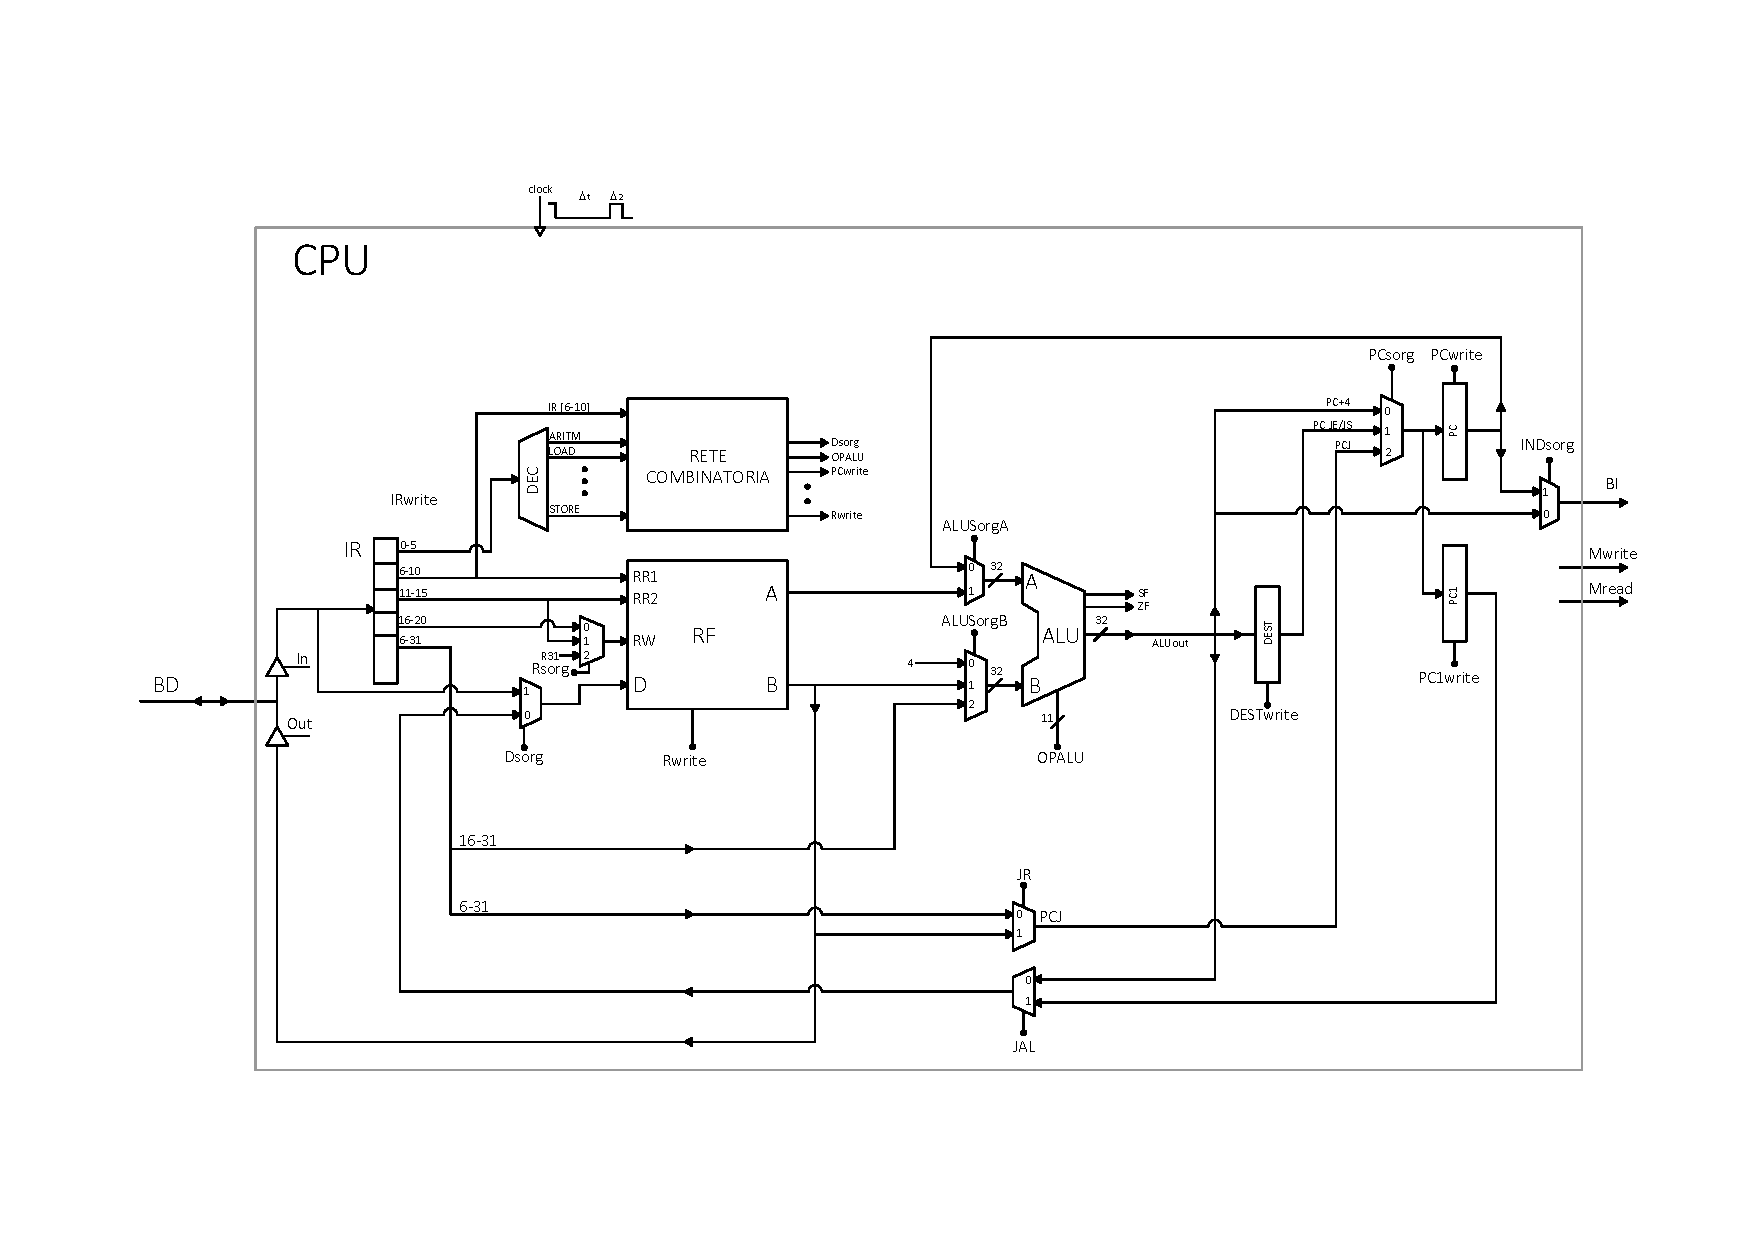
\includegraphics[width=\textwidth]{architettura_cpu}
\end{figure}
Un vantaggio che porta quest'architettura è che non necessita più di componenti come sommatore e memoria secondaria, dato che le diverse fasi dell'istruzione sono divise in diversi cicli di clock evitando conflitti di risorse.

\begin{itemize}
    \item Fetch:
        Dalla memoria viene letta l'istruzione indicata dal program counter. L'ALU incrementa il valore di quest'ultima per leggere la prossima istruzione al ciclo successivo.
    \item Decode:
        Il codice operativo indicato dell'istruzione entra in \code{IR}, viene assegnato il valore ai registri \code{R1} ed \code{R2}. L'ALU viene impiegata per calcolare il registro destinazione.
        \\
        In caso di salto condizionato, si calcola ugualmente il valore dell'indirizzo di destinazione, senza verificare le condizioni del salto.
    \item Operazione Aritmetica:
        Esegue l'istruzione utilizzando i dati calcolati nelle fasi precedenti.
    \item Memory attraverso le istruzioni \lstinline{load} e \lstinline{store}: vengono abilitati i segnali dei buffer 3state per lettura o scrittura dalla memoria all'indirizzo \code{Rd} calcolato nelle fasi precedenti.
    \item Writeback:
        In caso di operazione aritmetica prendo il valore in uscita dell'ALU e lo riporto nella porta dati del register file.
        In caso di load, il valore di uscita della memoria viene riportato nella porta dati del register file.
        In caso di JAL PC1 (valore precedente di PC) entra nel register file.
\end{itemize}

Interfacce con l'esterno: bus di dati attraverso buffer 3-state, in uscita al bus degli indirizzi arriva o alu-out o pc.


%2.7

\subsubsection{Segnali di controllo architettura multiciclo}
La fase di instruction fetch, comune a tutte le istruzioni, richiede di leggere l'istruzione corrente dalla memoria ed
incrementare il program counter di 4. Per queste operazioni necessita dei segnali:

    \begin{tabular}{ll}
        \code{Mread}  & Memory Read\\
        \code{In}   & abilitazione buffer 3state\\
        \code{PCwrite} & program counter write\\
        \code{PC1write}& program counter 1 write\\
        \code{IRwrite} & instruction register write
    \end{tabular}
    \hspace{3em}
    \begin{tabular}{ll}
        \code{INDsorg  = 1}   &invia al buffer in uscita \code{PC}\\
        \code{ALUsorgA = 0}   &\code{PC} come ingresso \code{A} dell'ALU\\
        \code{ALUsorgB = 0}   &\code{4} come ingresso \code{B} dell'ALU\\
        \code{OPALU    = ADD} &operazione somma\\
        \code{PCsorg   = 0}   &aggiorna \code{PC} in  \code{PC + 4}
    \end{tabular}

Nella fase di decode è richiesto di decodificare il codice operativo, inviare i due registri sorgente al register file
e sfrutto l'ALU non utilizzata per calcolare in anticipo l'indirizzo di destinazione gli eventuali salti condizionati:

\begin{tabular}{ll}
    \code{DESTwrite} & abilitazione scrittura nel registro destinazione\\
    \code{ALUsorgA=0}& \code{PC} in ingresso \\
    \code{ALUsorbB=2}& \code{offset} dell'istruzione in ingresso \\
    \code{OPALU = ADD} & operazione somma
\end{tabular}

Passate queste due fasi, comuni a tutte le operazioni, vi è una differenziazione a seconda del tipo di istruzione
contenuta in \code{IR}.

In caso di istruzioni aritmetiche, composte da execute (T3) e writeback (T5), in prima fase, sono richiesti i segnali \code{ALUsorgA=1}, \code{ALUsorgB=2} ed \code{OPALU} per specificare le operazioni dell'ALU; in fase di writeback:
\code{Rwrite} e \code{Rsorg = 0} per scrivere il contenuto del registro destinazione in \code{RF},
\code{DESTwrite = 0} per abilitare scrittura di \code{ALUout} in \code{dest}.
L'istruzione passa anche attraverso una fase di memory (T4) ma vengono solamente mantenuti i valori dei segnali in T3, mantenendo così \code{ALUout} costante.

In caso di load, nella fase di execute, viene calcolato l'indirizzo del dato in memoria \code{Rb + offset} (\code{ALUsorgA=1}, \code{ALUsorgB=2}, \code{OPALU=ADD}) e salvato in \code{Rdest}.
In fase T4, sono tenuti costanti i segnali in T3, inoltre \code{INDsorg = 0} e \code{Mr =1} per leggere il valore del dato all'indirizzo di memoria calcolato precedentemente.
A T5 viene salvato in \code{Rd} il dato letto dalla memoria \code{In=1} per mettere il bus dei dati in ingresso, viene abilitato \code{Rwrite} per abilitare la scrittura al register file.
\code{Rsorg=1} e \code{Dsorg=1} per scrivere il registro \code{Rd} il dato proveniente dalla memoria.

In caso di store, i segnali nella fase di execute sono identici a quelli della load, ma eseguo \code{INDsorg=0} uno step in anticipo, per avere il segnale stabile alla fase successiva e \code{Out=1}.
In T4 \code{Mw=1} per scrivere in memoria. Non ha una fase di writeback.

I salti condizionati richiedono solo un ciclo di completamento, in quanto l'indirizzo di destinazione è già calcolato nella fase precedente, è necessario solo da abilitare \code{PCwrite} in caso la condizione di salto sia verificata.
(\code{ALUsorgA = 1}, \code{ALUsorgB=1}, \code{OPALU=SUB}) \code{PCsorg=1} è richiesto per selezionare \code{DEST} come ingresso a PC.

In caso di salti incondizionati è presente la sola fase T3 con \code{PCwrite=1} e \code{PCsorg=2}.

L'ultimo caso \lstinline{jal}, è del tutto identico ad un salto condizionato, solo che viene seguito da una fase di
writeback, in cui salvare \code{PC1} in \code{R31}.
\subsection{Prestazioni dell'architettura multiciclo}
\begin{minipage}[t]{.66\textwidth}
    \vspace{0pt}
    Diversamente dall'architettura monociclo in cui $\tmono$ dipende dall'istruzione più lenta, il tempo $\tmulti$ dipende dallo
    stadio più lento.
    Prendendo come riferimento la tabella dei tempi di esecuzione dell'architettura monociclo (vedi pagina
    \pageref{tab:tempi_esecuzione_monociclo}), ne consegue $\tmulti =30$

    Confrontando le varie fasi ottengo chiaramente che i tempi di esecuzione delle singole istruzioni, ed il tempo di
    esecuzione medio è peggiore. Questo è dovuto ai $30ns$ della fase di fetch, che occupano più di 1/3 del tempo di
    esecuzione di una singola istruzione.
\end{minipage}
\begin{minipage}[t]{.33\textwidth}
    \footnotesize
    \let\fs\tiny
    \vspace{-2em}
    \begin{center}
        \begin{tabu}{|c|c|r|r|}
            \hline
            \rowfont{\bfseries\centering}
            Name & cck & Time & Usage \\
            \hline
            \hline
            Aritm  & 5& 150ns &40\fs\%\\
            \hline
            Load & 5& 150ns   &25\fs\%\\
            \hline
            Store & 4& 120ns  &10\fs\%\\
            \hline
            JE/JS& 3& 90ns    &12\fs\%\\
            \hline
            JMP/JR& 3& 90ns   &6\fs\%\\
            \hline
            JAL& 5& 150ns     &2\fs\%\\
            \hline
        \end{tabu}
    \end{center}
\end{minipage}

\subsection{Miglioramenti architettura multiciclo}
L'architettura multiciclo per come vista sino ad ora è inefficiente, per migliorarla ci possono essere diversi modi:
\begin{itemize}
    \item Ridurre il periodo di clock, introducendo salti di attesa per le fasi più lunghe
    \item Sfruttare le componenti inutilizzate, calcolando in anticipo operazioni richieste in fasi successive
    \item Unire fasi distinte e modificare opportunamente il segnale di clock
\end{itemize}
\subsubsection{Aumento granularità del clock}
Avendo preso $\tmulti$ uguale al tempo d'accesso alla memoria, nelle fasi in cui essa è inutilizzata, c'è spreco di
tempo. L'ideale per questa architettura sarebbe che tutti gli stadi richiedano approssimativamente lo stesso tempo di
esecuzione.
Prendendo ad esempio $\tmulti=12$ (tempo dell'ALU), gli stadi di accesso alla memoria richiederanno 3 cicli di clock
($12\cdot 3 > 30$).

Svolgendo i calcoli otteniamo un tempo medio di $86.88ns$, migliore rispetto al precedente, ma ancora più lento rispetto
agli $82ns$ dell'architettura monociclo.

Osservando che con $\tmulti=12$ nelle fasi di memoria rimane uno spreco di $36-3\cdot 12=6ns$ riduciamo ancora la
granularità di clock a $\tmulti=5ns$ (fase più veloce: decodifica del writeback)
saranno richiesti quindi 6 cicli di clock per le fasi che fanno accesso alla memoria, e 3 per le fasi di ALU.
Il tempo medio per istruzione si riduce a $75.65ns$, migliore rispetto al caso precedente e dell'architettura monociclo.
\subsubsection{Anticipazione delle operazioni}
Partiamo dall'osservazione che in T2 si esegue un passo che serve solo a JE/JS. Possiamo quindi differenziare la fase T2
a seconda dell'istruzione. Inoltre, dato che il periodo è sufficientemente lungo, possiamo unire più istruzioni in un
unico ciclo di clock:

\begin{itemize}
    \item Per operazioni aritmetiche, dopo il fetch, richiedono una decodifica ed un operazione dell'ALU, con un totale
        di $5 + 12 + 5=22ns$ sufficiente da eseguirle nell'unica fase T2
    \item Per load il calcolo dell'indirizzo può essere fatto in T2, la lettura della memoria in T3 e scrittura nel
        registro destinazione in T4, tagliando un ciclo di clock.
    \item L'operazione di store, esattamente come per la load, anticipiamo il calcolo dell'indirizzo sorgente in T2,
        quindi la scrittura in memoria è effettuabile immediatamente all'istante T3.
    \item In JMP/JS è possibile aggiornare PC direttamente in T2
    \item In JAL è possibile aggiornare PC e la scrittura in R31. PC1 non è più necessario.
\end{itemize}

Il tempo di esecuzione medio è $81.60ns$, migliore della versione multiciclo originale e circa la stessa velocità
dell'architettura monociclo.

Aumentando la granularità di clock in quest'architettura, ipotizzando un $\tmulti=6 ns$ (dato che IF e ME richiedono
$6ns$), otteniamo un tempo medio di $64.76ns$ migliore del $21\%$ rispetto alla monociclo.


\end{document}
